\pgfplotsset{
width=0.9\linewidth,
height=0.5\linewidth,
axis line style={color=Gray},
every axis label/.append style={font=\scriptsize},
every tick label/.append style={font=\scriptsize, Gray},
major grid style={Gray!20, very thin},
minor grid style={Gray!20, very thin},  
}
\tikzstyle{every pin}=[
fill=none,
draw=none,
font=\small,
]
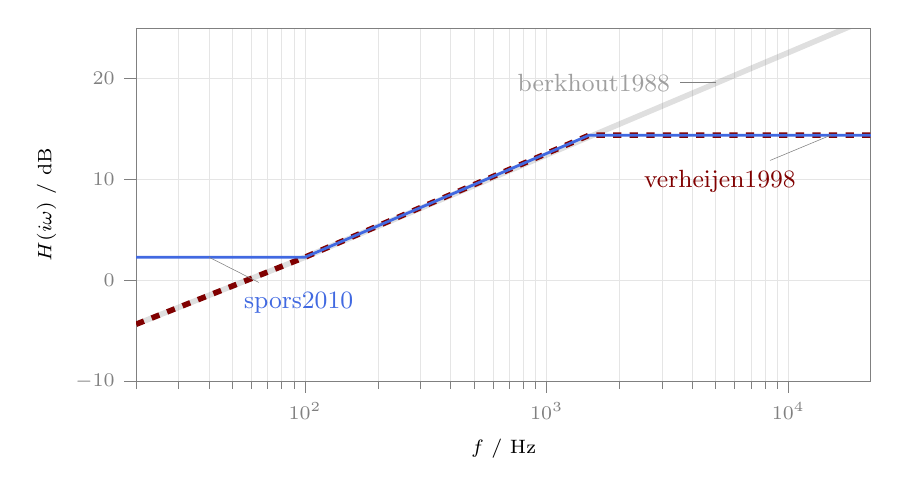
\begin{tikzpicture}
\begin{semilogxaxis}[
grid=both, tick align=outside, tickpos=left,
xmin=20, xmax=22000, ymin=-10, ymax=25,
ylabel near ticks,
xlabel={$f$ / Hz}, ylabel={$\Abs{H(i\omega)}$ / dB},
]
\addplot[line width=2pt, color=Gray, opacity=0.25] coordinates {
(20, -4.36) (100, 2.29) (22000, 26.05)
};
\addplot[line width=2pt, dashed, color=Maroon] coordinates {
(20, -4.36) (100, 2.29) (1500, 14.39) (22000, 14.39)
};
\addplot[line width=1pt, color=RoyalBlue, opacity=1] coordinates {
(20, 2.29) (100, 2.29) (1500, 14.39) (22000, 14.39)
};
\node [coordinate, pin=left:{\textcolor{Gray!75}{\citep{berkhout1988}}}]
at (axis cs:5000, 19.62) {};
\node [coordinate, pin=below left:{\textcolor{Maroon}{\citep{verheijen1998}}}]
at (axis cs:15000, 14.39) {};
\node [coordinate, pin=below right:{\textcolor{RoyalBlue}{\citep{spors2010}}}]
at (axis cs:40, 2.29) {};
\end{semilogxaxis}
\end{tikzpicture}